\documentclass[sigchi, review]{acmart}

\usepackage{booktabs} % For formal tables


% Copyright
%\setcopyright{none}
%\setcopyright{acmcopyright}
%\setcopyright{acmlicensed}
%\setcopyright{rightsretained}
%\setcopyright{usgov}
%\setcopyright{usgovmixed}
%\setcopyright{cagov}
\setcopyright{licensedcagov}
%\setcopyright{cagovmixed}
%\setcopyright{licensedothergov}

% DOI
\acmDOI{10.475/123_4}

% ISBN
\acmISBN{123-4567-24-567/08/06}

%Conference
\acmConference[WOODSTOCK'97]{ACM Woodstock conference}{July 1997}{El
  Paso, Texas USA}
\acmYear{1997}
\copyrightyear{2016}

\acmPrice{15.00}


\begin{document}
\title{SIG Proceedings Paper in LaTeX Format}
\titlenote{Produces the permission block, and
  copyright information}
\subtitle{Extended Abstract}
\subtitlenote{The full version of the author's guide is available as
  \texttt{acmart.pdf} document}

\author{Ben Trovato}
\authornote{Dr.~Trovato insisted his name be first.}
\orcid{1234-5678-9012}
\affiliation{%
  \institution{Institute for Clarity in Documentation}
  \streetaddress{P.O. Box 1212}
  \city{Dublin}
  \state{Ohio}
  \postcode{43017-6221}
}
\email{trovato@corporation.com}

\author{G.K.M. Tobin}
\authornote{The secretary disavows any knowledge of this author's actions.}
\affiliation{%
  \institution{Institute for Clarity in Documentation}
  \streetaddress{P.O. Box 1212}
  \city{Dublin}
  \state{Ohio}
  \postcode{43017-6221}
}
\email{webmaster@marysville-ohio.com}

\author{Lars Th{\o}rv{\"a}ld}
\authornote{This author is the
  one who did all the really hard work.}
\affiliation{%
  \institution{The Th{\o}rv{\"a}ld Group}
  \streetaddress{1 Th{\o}rv{\"a}ld Circle}
  \city{Hekla}
  \country{Iceland}}
\email{larst@affiliation.org}

\author{Valerie B\'eranger}
\affiliation{%
  \institution{Inria Paris-Rocquencourt}
  \city{Rocquencourt}
  \country{France}
}
\author{Aparna Patel}
\affiliation{%
 \institution{Rajiv Gandhi University}
 \streetaddress{Rono-Hills}
 \city{Doimukh}
 \state{Arunachal Pradesh}
 \country{India}}
\author{Huifen Chan}
\affiliation{%
  \institution{Tsinghua University}
  \streetaddress{30 Shuangqing Rd}
  \city{Haidian Qu}
  \state{Beijing Shi}
  \country{China}}

\author{Charles Palmer}
\affiliation{%
  \institution{Palmer Research Laboratories}
  \streetaddress{8600 Datapoint Drive}
  \city{San Antonio}
  \state{Texas}
  \postcode{78229}}
\email{cpalmer@prl.com}

\author{John Smith}
\affiliation{\institution{The Th{\o}rv{\"a}ld Group}}
\email{jsmith@affiliation.org}

\author{Julius P.~Kumquat}
\affiliation{\institution{The Kumquat Consortium}}
\email{jpkumquat@consortium.net}

% The default list of authors is too long for headers.
\renewcommand{\shortauthors}{B. Trovato et al.}


\begin{abstract}
This paper provides a sample of a \LaTeX\ document which conforms,
somewhat loosely, to the formatting guidelines for
ACM SIG Proceedings.
\end{abstract}

%
% The code below should be generated by the tool at
% http://dl.acm.org/ccs.cfm
% Please copy and paste the code instead of the example below.
%
\begin{CCSXML}
<ccs2012>
 <concept>
  <concept_id>10010520.10010553.10010562</concept_id>
  <concept_desc>Computer systems organization~Embedded systems</concept_desc>
  <concept_significance>500</concept_significance>
 </concept>
 <concept>
  <concept_id>10010520.10010575.10010755</concept_id>
  <concept_desc>Computer systems organization~Redundancy</concept_desc>
  <concept_significance>300</concept_significance>
 </concept>
 <concept>
  <concept_id>10010520.10010553.10010554</concept_id>
  <concept_desc>Computer systems organization~Robotics</concept_desc>
  <concept_significance>100</concept_significance>
 </concept>
 <concept>
  <concept_id>10003033.10003083.10003095</concept_id>
  <concept_desc>Networks~Network reliability</concept_desc>
  <concept_significance>100</concept_significance>
 </concept>
</ccs2012>
\end{CCSXML}

\ccsdesc[500]{Computer systems organization~Embedded systems}
\ccsdesc[300]{Computer systems organization~Redundancy}
\ccsdesc{Computer systems organization~Robotics}
\ccsdesc[100]{Networks~Network reliability}


\keywords{ACM proceedings, \LaTeX, text tagging}

\begin{teaserfigure}
  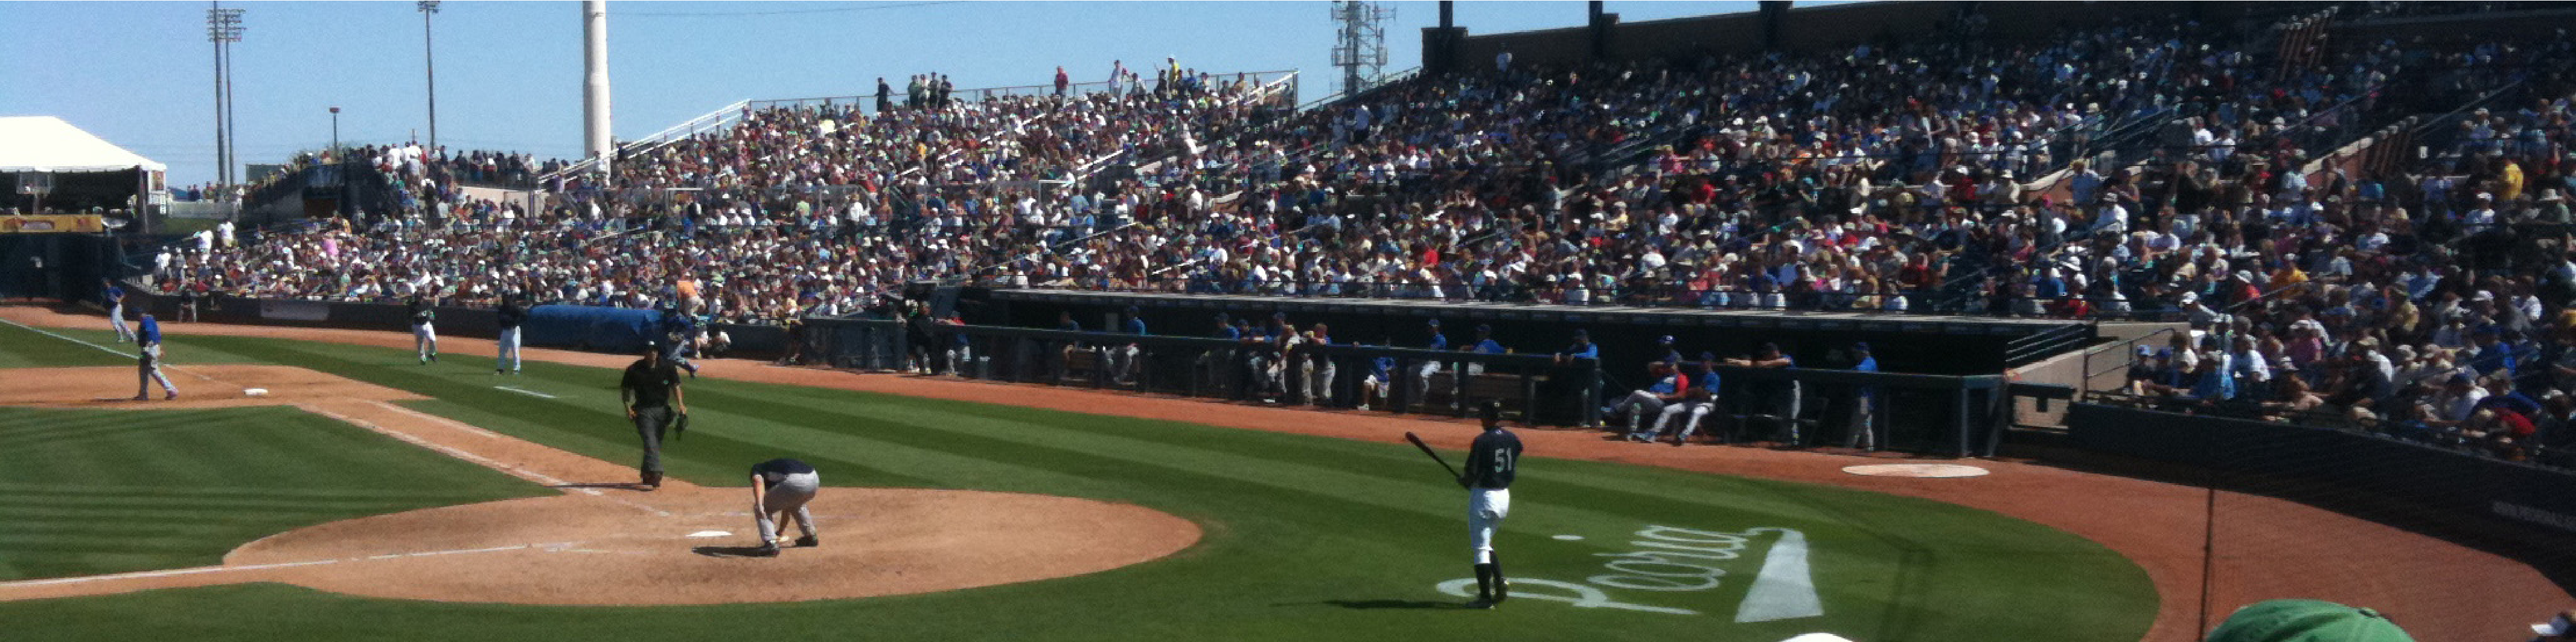
\includegraphics[width=\textwidth]{sampleteaser}
  \caption{This is a teaser}
  \label{fig:teaser}
\end{teaserfigure}


\maketitle


\section{Introduction}
Part of speech (POS) tagging is the key topic for information retrieval area to extract the valuable information that is used for classification, clustering etc. from any natural languages. 


In this paper, it is aimed to automatically model the steps of a certain task by using text data which is easily accessible from the internet and to create methods and tool that can help people since there are many recipe documents and videos available on the internet,  in this paper, working area is selected as cooking recipes. POS tagging is important that  it constructs a description a set of instructions of a recipes which forms content based text analysis of our work.

In this paper we describe a rule-based tagger which
performs as well as taggers based upon probabilistic
models. The rule-based tagger overcomes the limitations
common in rule-based approaches to language processing:
it is robust, and the rules are automatically acquired.
In addition, the tagger has many advantages
over stochastic taggers, including: a vast reduction in
stored information required, the perspicuity of a small
set of meaningful rules as opposed to the large tables
of statistics needed for stochastic taggers, ease of finding
and implementing improvements to the tagger, and
better portability from one tag set or corpus genre to
another. 

\section{Related Works}
Algorithmic processing of training texts and / or commands expressed in natural language has long been an interesting question (Harnad, 1990). In this problem, the artificial intelligence agent (such as a robot) is trying to learn the operations corresponding to symbols that are expressed in a field. The system is expected to automatically interact with definitions in the physical world as symbols to interact with objects and objects. We obtained through www.allrecipes.com

Chen and Mooney (2011) have developed a system that can act according to the expressions expressed in natural language in the system they developed. Based on the reinforced learning methods, the system can translate the sentences into natural language by using the information in the location (such as the objects on the wall) and the state flow that is modeled. As can be seen from these studies in the literature, reinforcement learning techniques are used in problems where the current situation can be modeled more clearly.
A slightly different problem is Kushman et al. (2014) developed a similar method for solving problems expressed in mathematical texts. According to this method, the system is mapping the problem described in the text to a set of equations and producing the result. To learn the method, we use a training set marked at different levels. Equations that can be created in the system can be given or can be learned only when the last answer is given. In the method they developed, the solution is defined as diagrams, and a probability model that maps the information given in the text to the diagram is developed. Of course, it is necessary that the structure of the questionnaire is similar and that all of them can be transferred to the equation diagram.

Recipes can also be thought of as a set of steps that must be followed. From this point of view, there are common aspects to the problems described above. The most important difference is that it is difficult to convert the media knowledge to a reward function to provide reinforcement learning. The biggest reason for this is that it is difficult to model the correct sequence of operations that can be done while cooking. To overcome this problem in the processing of recipes, three different basic approaches are striking. The first is knowledge-based methods that are dependent on previously created knowledge vocabulary, the second is those using supervised learning methods, and the third is unsupervised learning and extracting a specific model from the data in the compilation. The first approach involves all the recipes, contents, tools and processes, and methods that can show the relationship between them. In the second approach, it is necessary to generate the data with the equivalent of the text for the training compilation. In the third category, transductive learning is performed according to the solutions given, ie it is not possible to classify the given samples and to process new ones.

\subsection{Information Based Methods}
Walter et al. (2011) describes a method of generating flow diagrams from recipe texts, extracting recipe statements as material, processing and finishing conditions. Based on this information, a flow diagram is created. This method requires pre-tagged sentences and a dictionary that holds all of these tags.

Another problem that may be related is the creation of an information dictionary. Gaiilard et al. (2012) foods and their relationships with a Wiki-style method. Its approach basically consists of 6 hierarchies; diet and mealtime according to different features categorize the food. With this approach it is possible to adapt a new recipe or an existing recipe.

Although food-related ontology is increasingly detailed, these methods often fail to adapt to dynamic language and variety. Thus, when ontology methods are used alone, successful results are achieved for some data sets, but success is often low. Moreover, in order to adapt these methods to a different language, ontologies should be structured in accordance with other languages.


\subsection{Supervised Learning Methods}
One of the most important features of tutorial learning techniques is the target description model. Basically, the information that this model needs to be able to show is where the processes described in the steps are done on which materials and where the output of this step is used. Some of these associations show in the tree structure (Jermsurawong and Habash, 2015), while some researchers show it in a non-cyclic manner (Malmoud et al., 2014). It is possible that this notation can both express all the recipes and learn it automatically.
Jermsurawong and Habash (2015) defined a representation in the tree data structure that stores food items and their relationships over the description steps. This demonstration can show which step of the recipes is related to which steps and materials.

Malmoud et al. (2014) sees text in recipes as a Markov Decision Process problem by expanding semantic role labeling. It holds two things between the process and the material. The purpose of this relationship is to demonstrate the processes within the training that cause these situations to occur.
Mori et al. (2014) created a labeling tool by showing recipes as non-cyclic charts in their initial work. With this tool, the recipe created a graph that indicates the skis over the text. The given Japanese recipes first extract the word segmentation, locate the words in the clan's tasks, label the named entities, and finally construct the predicate-argument structure.
In order to resolve the uncertainties in the contents, Erica Greene (2016) tagged a total of 187,000 sentences for labeling and edited the tags of the words in the table of contents using the Conditional Random Fields method.


\subsection{Unsupervised Learning Methods}
In 2015, Kiddon et al. (2015) has developed a method of learning without a teacher for the processing of recipes. Unlike previous works, this method learns the linkages of the line by using different parameters according to the variables in the system and using the expectation maximization method. Since this model is constructed according to the definition in the drawing, it is not possible to learn the features of an extragalactic recipe. In this respect, it is a transduction method, all the recipes to be processed have to be obtained at the model learning time. Moreover, the generated data model has a high number of implicit variables because it defines both the verbs, the contents, and the content of the contents in relation to the steps as one of the parameters of the model. When such high numbered models are learned, they can be found in a high number of local maxima, which prevents the optimum model from being found.
It is intended to remove them as to which action is associated with the material, removing the flow of the recipe as a whole. These methods are inspired by semantic spaces used in text mining and meaning spaces that show word meaning relations. By using these material spaces, it is possible to determine which materials can be replaced instead of which materials. Nedovic (2013) used a similar method to define a method of learning materials for different types of food. Latent Dirichlet Allocation (LDA) and Deep Belief Networks (DBN) are used in the method. It has been seen that the output of the system can group materials according to the foods in different kitchens. A similar study has been proposed by Achananuparp and Weber (2016) to produce safer food recommendations in meals. In this method, Singular Value Decomposition (SVD) method, which is widely used for extracting word meaning relations, is used.

\section{Experimental Setup}
As seen in the literature, there are many methods aiming at revealing the relationship between the description texts and the contents of the description texts, the sequence of the process flow and the situations that occur during the actions and showing them with the models by many different methods. The texts should be easily perceivable by the computer by passing 1830 recipes we obtained through www.alrecipes.com through certain operations.

Using NLTK libraries, each of the recipes was first converted into a clean text by separating individual recipes and separating them into words, punctuation, and meaningless words.  (names, categories, contents, descriptions, and comments). Then each recipe is divided into sentences for labelling.

\begin{algorithm}
\caption{Data Retrieval and Preprocessing Overview}
\label{alg:generator}
\SetKwProg{ReadProcessData}{Function \emph{ReadProcessData}}{}{end}

\ReadProcessData{CvsFiles data}{
     \ForAll{eachRecipe $c$ in data}{
(ingredients, direction) = readDataFromCSVfile($c$)
ingredientsNewTag = calculateTAGWithCRF(ingredients)
tokenizeddirection = tokenizesentence(direction)
taggedDirection = calculateTagsWithPOSTag(tokenizedDirection)
taggedDirection = updateTagAfterCRF(taggedDirection, ingredientsNewTag)
      
     }
     build pivot's fieldContext $fc$\;
     EmitClassName\;
     EmitFields($fc$)\;
     EmitMethods($fc$)\;
}
\end{algorithm}


\begin{algorithm}
\caption{Pos Tagging Overview}
\label{alg:generator}
\SetKwProg{generate}{Function \emph{generate}}{}{end}

Map store=new Map(obj, queue)\;
\generate{Object pivot}{
     \ForAll{child $c$ in pivot}{
     \If{ $c$'s FieldContext is not set and $c$ is fusible}{
          generate($c$)\;
      }
     }
     build pivot's fieldContext $fc$\;
     EmitClassName\;
     EmitFields($fc$)\;
     EmitMethods($fc$)\;
}
\end{algorithm}


\begin{algorithm}
\caption{Graph Generation and Validation}
\label{alg:generator}
\SetKwProg{generate}{Function \emph{generate}}{}{end}

Map store=new Map(obj, queue)\;
\generate{Object pivot}{
     \ForAll{child $c$ in pivot}{
     \If{ $c$'s FieldContext is not set and $c$ is fusible}{
          generate($c$)\;
      }
     }
     build pivot's fieldContext $fc$\;
     EmitClassName\;
     EmitFields($fc$)\;
     EmitMethods($fc$)\;
}
\end{algorithm}

\subsection{Labelling}
Using the NLTK library, labeling was done according to the culled state (VB, NN, ADJ, etc.) that each of the belts passed. As a result of the labeling made, "I can chopped green chile peppers" in the table of contents is labeled as below in TABLE 1.

\begin{table}[]
\centering
\caption{Tags}
\label{my-label}
\begin{tabular}{|l|l|l|l|l|l|}
\hline
I   & can & chopped & green & chile & peppers \\ \hline
ADJ & NN  & VB      & NN    & NN    & NN      \\ \hline
\end{tabular}
\end{table}

As can be seen in Table 1, it does not allow me to know that the word "life" is a unit of measure, "1" actually tells the quantity, and that the words "green" and "choped" are actually interpretations of a "papers" word.

The challenge of parsing the recipe is to be able to distinguish content components from component cues. Erica Greene (2016) has trained 171,244 sets (labeled as UNIT, QUANTITY, COMMENT and OTHER) with the very specific set of CRF ++ (Conditional Random Fields) method she has created to solve this problem and has been able to label the contents portion probabilistically with a newly given description. Let us have the sentence "1 teaspoon sugar". The model is using 171,224 tagged data to learn a model that can predict the tag sequence for any sentence we have given to it, even though we have never seen this component count before. It approaches this by modeling the conditional probability of a set of labels.

p (UNIT UNIT UNIT| "1 teaspoon sugar")

p (QUANTITY UNIT UNIT| "1 teaspoon sugar")

p (UNIT QUANTITY UNIT| "1 teaspoon sugar")

p (UNIT UNIT QUANTITY "1 teaspoon sugar")

p (UNIT QUANTITY QUANTITY "1 teaspoon sugar")

p (QUANTITY QUANTITY QUANTITY | "1 teaspoon sugar")

p (UNIT QUANTITY NAME| "1 teaspoon sugar")

...

As mentioned above, it calculates all the probabilities that can be labeled "1 teaspoon sugar". The beauty of the linear-chain CRF model makes some conditional independence assumptions that allow us to use dynamic programming to efficiently search the area of all possible label sequences. As a result, we have re-tagged our data with Erica Greene (2016), and the result is shown in TABLE 2. The results are shown in Table 2, which shows the best label sequence at a time that is linear with the number of second.


\begin{table}[]
\centering
\caption{Tags}
\label{my-label}
\begin{tabular}{|l|l|l|l|l|l|}
\hline
I   & can & chopped & green & chile & peppers \\ \hline
QT & UNIT  & CMMT      & CMMT    & NAME    & NAME      \\ \hline
\end{tabular}
\end{table}

It was observed that 450 of 171.224 labeled samples were separated and tested and 76 percentage correctly tagged.


\subsection{Calculation of Proximity}
Kiddon et al. (2015), some words are not in the table of contents, but more than one is meant. (Eg mixture, them) Kiddon et al. (2015) defines this as a hidden object. He has created a probabilistic model to make hidden objects clear. In order to reveal these hidden objects, we present a relationship between the words 'NAME' in this action and its contents. In fact, each word is represented as a vector and we calculate the cosine similarity between them.

Using the Word2Vec library that displays 3.5 billion words created by a working group led by Tomas Mikolov (Google) as a 300-dimensional vector vocabulary, the words that pass through the intellectual part and are labeled 'NAME' have been converted into a 300-dimensional vector.

In the recipe sentence set, phrases without any word labeled 'NAME' are removed. When the words labeled as 'VB' are extracted, all the words are converted into 300 dimensional vectors and the averages are taken. Because the other words around the word tagged by "VB" can also provide us with information about what materials the hidden object contains. If you only go through the actions, you will be made a comment by looking at the similarity of only two calves. However, the sentence can sometimes contain words that characterize the words in the contents. Let's take a look at "Cook the mixture until caramelized". It is labeled as "cook-VB". When we look at the similarity of the cosine with the contents, it is seen that almost all of them resemble to each other. However, when the complex average of sentence is taken, "caramelized" word is included. And the result is more similar to "Onion" and "sugar". Taking the average of the blame for this reason actually brings us closer to the right conclusion.

\subsubsection{Inline (In-text) Equations}
A formula that appears in the running text is called an
inline or in-text formula.  It is produced by the
\textbf{math} environment, which can be
invoked with the usual \texttt{{\char'134}begin\,\ldots{\char'134}end}
construction or with the short form \texttt{\$\,\ldots\$}. You
can use any of the symbols and structures,
from $\alpha$ to $\omega$, available in
\LaTeX~\cite{Lamport:LaTeX}; this section will simply show a
few examples of in-text equations in context. Notice how
this equation:
\begin{math}
  \lim_{n\rightarrow \infty}x=0
\end{math},
set here in in-line math style, looks slightly different when
set in display style.  (See next section).



\subsubsection{Display Equations}
A numbered display equation---one set off by vertical space from the
text and centered horizontally---is produced by the \textbf{equation}
environment. An unnumbered display equation is produced by the
\textbf{displaymath} environment.

Again, in either environment, you can use any of the symbols
and structures available in \LaTeX\@; this section will just
give a couple of examples of display equations in context.
First, consider the equation, shown as an inline equation above:
\begin{equation}
  \lim_{n\rightarrow \infty}x=0
\end{equation}
Notice how it is formatted somewhat differently in
the \textbf{displaymath}
environment.  Now, we'll enter an unnumbered equation:
\begin{displaymath}
  \sum_{i=0}^{\infty} x + 1
\end{displaymath}
and follow it with another numbered equation:
\begin{equation}
  \sum_{i=0}^{\infty}x_i=\int_{0}^{\pi+2} f
\end{equation}
just to demonstrate \LaTeX's able handling of numbering.

\subsection{Citations}
Citations to articles~\cite{bowman:reasoning,
clark:pct, braams:babel, herlihy:methodology},
conference proceedings~\cite{clark:pct} or maybe
books \cite{Lamport:LaTeX, salas:calculus} listed
in the Bibliography section of your
article will occur throughout the text of your article.
You should use BibTeX to automatically produce this bibliography;
you simply need to insert one of several citation commands with
a key of the item cited in the proper location in
the \texttt{.tex} file~\cite{Lamport:LaTeX}.
The key is a short reference you invent to uniquely
identify each work; in this sample document, the key is
the first author's surname and a
word from the title.  This identifying key is included
with each item in the \texttt{.bib} file for your article.

The details of the construction of the \texttt{.bib} file
are beyond the scope of this sample document, but more
information can be found in the \textit{Author's Guide},
and exhaustive details in the \textit{\LaTeX\ User's
Guide} by Lamport~\shortcite{Lamport:LaTeX}.

This article shows only the plainest form
of the citation command, using \texttt{{\char'134}cite}.

Some examples.  A paginated journal article \cite{Abril07}, an enumerated
journal article \cite{Cohen07}, a reference to an entire issue \cite{JCohen96},
a monograph (whole book) \cite{Kosiur01}, a monograph/whole book in a series (see 2a in spec. document)
\cite{Harel79}, a divisible-book such as an anthology or compilation \cite{Editor00}
followed by the same example, however we only output the series if the volume number is given
\cite{Editor00a} (so Editor00a's series should NOT be present since it has no vol. no.),
a chapter in a divisible book \cite{Spector90}, a chapter in a divisible book
in a series \cite{Douglass98}, a multi-volume work as book \cite{Knuth97},
an article in a proceedings (of a conference, symposium, workshop for example)
(paginated proceedings article) \cite{Andler79}, a proceedings article
with all possible elements \cite{Smith10}, an example of an enumerated
proceedings article \cite{VanGundy07},
an informally published work \cite{Harel78}, a doctoral dissertation \cite{Clarkson85},
a master's thesis: \cite{anisi03}, an online document / world wide web
resource \cite{Thornburg01, Ablamowicz07, Poker06}, a video game (Case 1) \cite{Obama08} and (Case 2) \cite{Novak03}
and \cite{Lee05} and (Case 3) a patent \cite{JoeScientist001},
work accepted for publication \cite{rous08}, 'YYYYb'-test for prolific author
\cite{SaeediMEJ10} and \cite{SaeediJETC10}. Other cites might contain
'duplicate' DOI and URLs (some SIAM articles) \cite{Kirschmer:2010:AEI:1958016.1958018}.
Boris / Barbara Beeton: multi-volume works as books
\cite{MR781536} and \cite{MR781537}.

A couple of citations with DOIs: \cite{2004:ITE:1009386.1010128,
  Kirschmer:2010:AEI:1958016.1958018}.

Online citations: \cite{TUGInstmem, Thornburg01, CTANacmart}.


\subsection{Tables}
Because tables cannot be split across pages, the best
placement for them is typically the top of the page
nearest their initial cite.  To
ensure this proper ``floating'' placement of tables, use the
environment \textbf{table} to enclose the table's contents and
the table caption.  The contents of the table itself must go
in the \textbf{tabular} environment, to
be aligned properly in rows and columns, with the desired
horizontal and vertical rules.  Again, detailed instructions
on \textbf{tabular} material
are found in the \textit{\LaTeX\ User's Guide}.

Immediately following this sentence is the point at which
Table~\ref{tab:freq} is included in the input file; compare the
placement of the table here with the table in the printed
output of this document.

\begin{table}
  \caption{Frequency of Special Characters}
  \label{tab:freq}
  \begin{tabular}{ccl}
    \toprule
    Non-English or Math&Frequency&Comments\\
    \midrule
    \O & 1 in 1,000& For Swedish names\\
    $\pi$ & 1 in 5& Common in math\\
    \$ & 4 in 5 & Used in business\\
    $\Psi^2_1$ & 1 in 40,000& Unexplained usage\\
  \bottomrule
\end{tabular}
\end{table}

To set a wider table, which takes up the whole width of the page's
live area, use the environment \textbf{table*} to enclose the table's
contents and the table caption.  As with a single-column table, this
wide table will ``float'' to a location deemed more desirable.
Immediately following this sentence is the point at which
Table~\ref{tab:commands} is included in the input file; again, it is
instructive to compare the placement of the table here with the table
in the printed output of this document.


\begin{table*}
  \caption{Some Typical Commands}
  \label{tab:commands}
  \begin{tabular}{ccl}
    \toprule
    Command &A Number & Comments\\
    \midrule
    \texttt{{\char'134}author} & 100& Author \\
    \texttt{{\char'134}table}& 300 & For tables\\
    \texttt{{\char'134}table*}& 400& For wider tables\\
    \bottomrule
  \end{tabular}
\end{table*}
% end the environment with {table*}, NOTE not {table}!

It is strongly recommended to use the package booktabs~\cite{Fear05}
and follow its main principles of typography with respect to tables:
\begin{enumerate}
\item Never, ever use vertical rules.
\item Never use double rules.
\end{enumerate}
It is also a good idea not to overuse horizontal rules.


\subsection{Figures}

Like tables, figures cannot be split across pages; the best placement
for them is typically the top or the bottom of the page nearest their
initial cite.  To ensure this proper ``floating'' placement of
figures, use the environment \textbf{figure} to enclose the figure and
its caption.

This sample document contains examples of \texttt{.eps} files to be
displayable with \LaTeX.  If you work with pdf\LaTeX, use files in the
\texttt{.pdf} format.  Note that most modern \TeX\ systems will convert
\texttt{.eps} to \texttt{.pdf} for you on the fly.  More details on
each of these are found in the \textit{Author's Guide}.

\begin{figure}
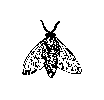
\includegraphics{fly}
\caption{A sample black and white graphic.}
\end{figure}

\begin{figure}
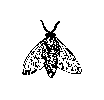
\includegraphics[height=1in, width=1in]{fly}
\caption{A sample black and white graphic
that has been resized with the \texttt{includegraphics} command.}
\end{figure}


As was the case with tables, you may want a figure that spans two
columns.  To do this, and still to ensure proper ``floating''
placement of tables, use the environment \textbf{figure*} to enclose
the figure and its caption.  And don't forget to end the environment
with \textbf{figure*}, not \textbf{figure}!

\begin{figure*}
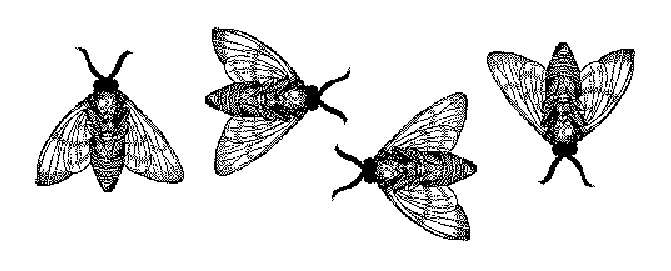
\includegraphics{flies}
\caption{A sample black and white graphic
that needs to span two columns of text.}
\end{figure*}


\begin{figure}
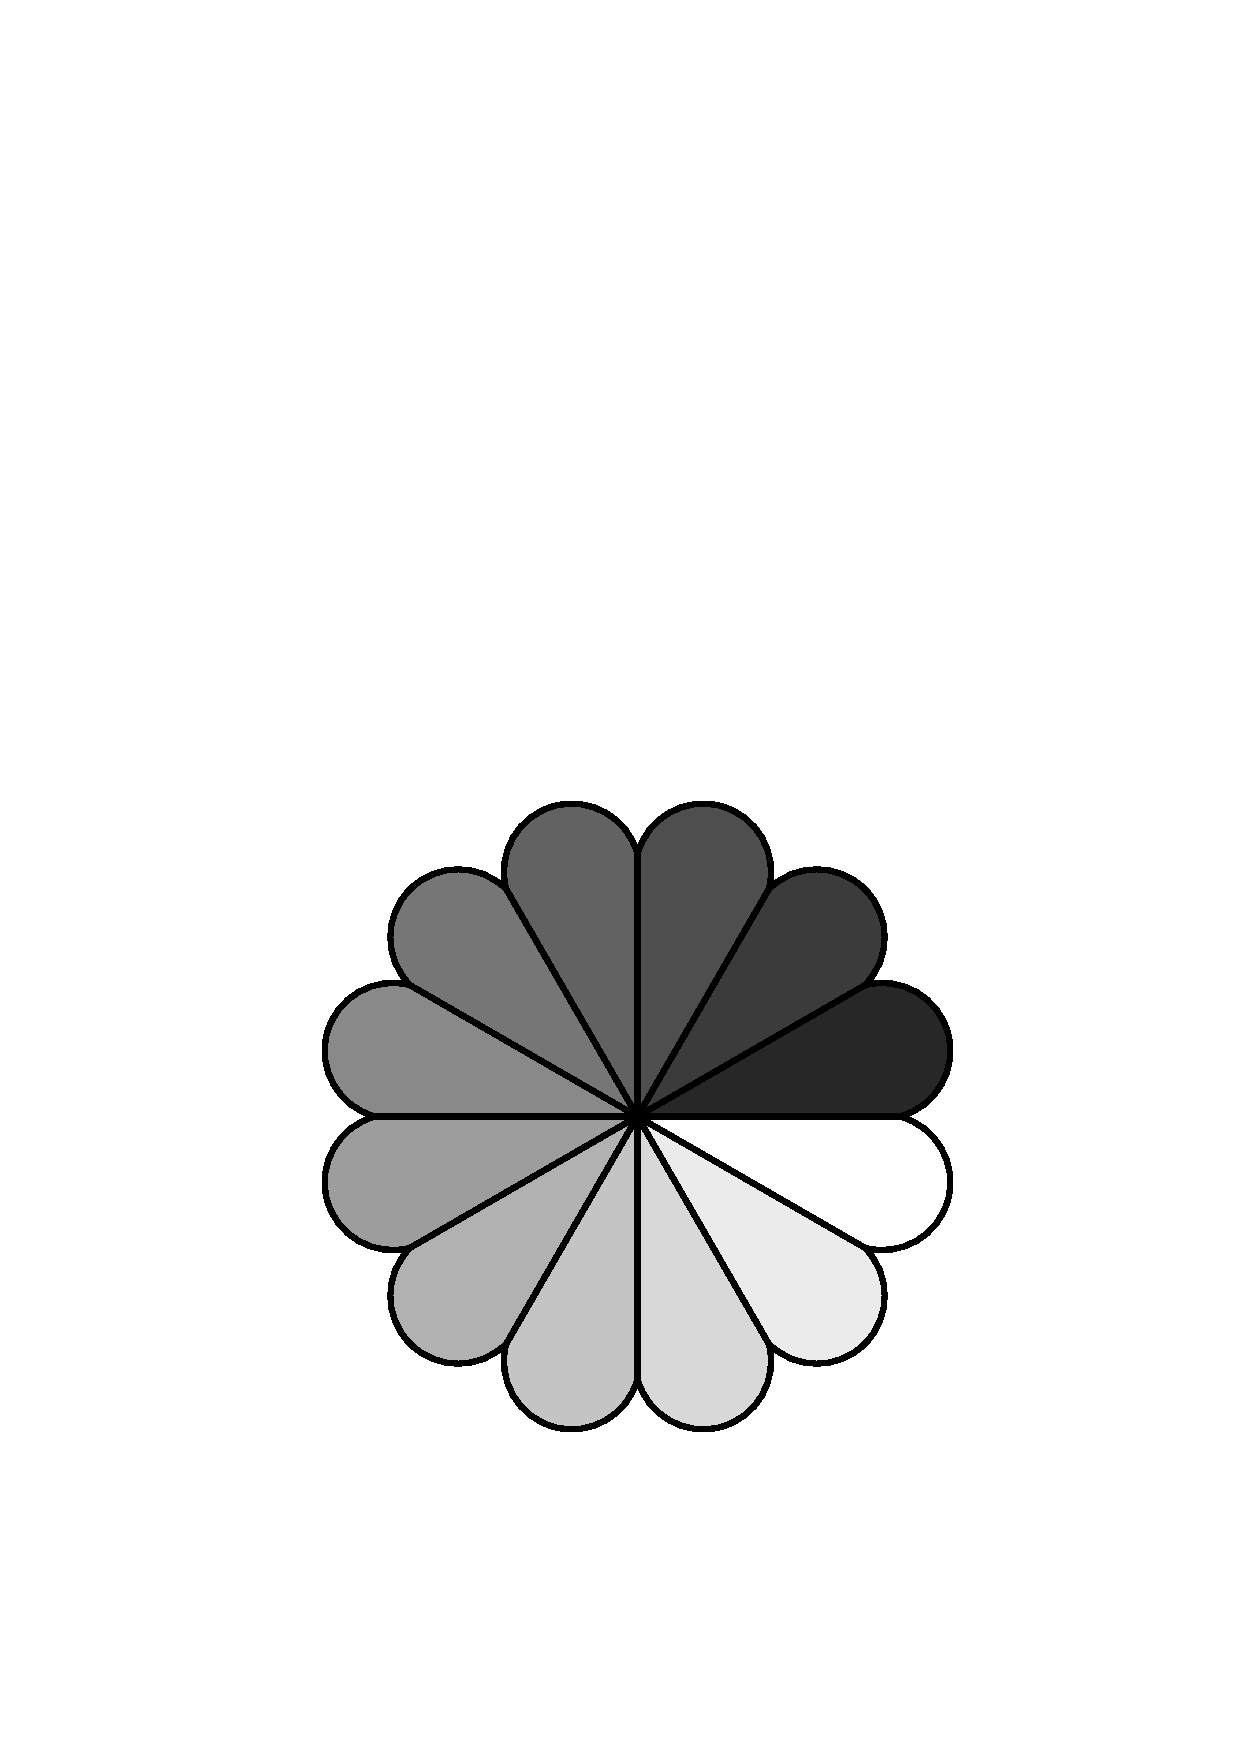
\includegraphics[height=1in, width=1in]{rosette}
\caption{A sample black and white graphic that has
been resized with the \texttt{includegraphics} command.}
\end{figure}

\subsection{Theorem-like Constructs}

Other common constructs that may occur in your article are the forms
for logical constructs like theorems, axioms, corollaries and proofs.
ACM uses two types of these constructs:  theorem-like and
definition-like.

Here is a theorem:
\begin{theorem}
  Let $f$ be continuous on $[a,b]$.  If $G$ is
  an antiderivative for $f$ on $[a,b]$, then
  \begin{displaymath}
    \int^b_af(t)\,dt = G(b) - G(a).
  \end{displaymath}
\end{theorem}

Here is a definition:
\begin{definition}
  If $z$ is irrational, then by $e^z$ we mean the
  unique number that has
  logarithm $z$:
  \begin{displaymath}
    \log e^z = z.
  \end{displaymath}
\end{definition}

The pre-defined theorem-like constructs are \textbf{theorem},
\textbf{conjecture}, \textbf{proposition}, \textbf{lemma} and
\textbf{corollary}.  The pre-defined de\-fi\-ni\-ti\-on-like constructs are
\textbf{example} and \textbf{definition}.  You can add your own
constructs using the \textsl{amsthm} interface~\cite{Amsthm15}.  The
styles used in the \verb|\theoremstyle| command are \textbf{acmplain}
and \textbf{acmdefinition}.

Another construct is \textbf{proof}, for example,

\begin{proof}
  Suppose on the contrary there exists a real number $L$ such that
  \begin{displaymath}
    \lim_{x\rightarrow\infty} \frac{f(x)}{g(x)} = L.
  \end{displaymath}
  Then
  \begin{displaymath}
    l=\lim_{x\rightarrow c} f(x)
    = \lim_{x\rightarrow c}
    \left[ g{x} \cdot \frac{f(x)}{g(x)} \right ]
    = \lim_{x\rightarrow c} g(x) \cdot \lim_{x\rightarrow c}
    \frac{f(x)}{g(x)} = 0\cdot L = 0,
  \end{displaymath}
  which contradicts our assumption that $l\neq 0$.
\end{proof}

\section{Conclusions}
This paragraph will end the body of this sample document.
Remember that you might still have Acknowledgments or
Appendices; brief samples of these
follow.  There is still the Bibliography to deal with; and
we will make a disclaimer about that here: with the exception
of the reference to the \LaTeX\ book, the citations in
this paper are to articles which have nothing to
do with the present subject and are used as
examples only.
%\end{document}  % This is where a 'short' article might terminate



\appendix
%Appendix A
\section{Headings in Appendices}
The rules about hierarchical headings discussed above for
the body of the article are different in the appendices.
In the \textbf{appendix} environment, the command
\textbf{section} is used to
indicate the start of each Appendix, with alphabetic order
designation (i.e., the first is A, the second B, etc.) and
a title (if you include one).  So, if you need
hierarchical structure
\textit{within} an Appendix, start with \textbf{subsection} as the
highest level. Here is an outline of the body of this
document in Appendix-appropriate form:
\subsection{Introduction}
\subsection{The Body of the Paper}
\subsubsection{Type Changes and  Special Characters}
\subsubsection{Math Equations}
\paragraph{Inline (In-text) Equations}
\paragraph{Display Equations}
\subsubsection{Citations}
\subsubsection{Tables}
\subsubsection{Figures}
\subsubsection{Theorem-like Constructs}
\subsubsection*{A Caveat for the \TeX\ Expert}
\subsection{Conclusions}
\subsection{References}
Generated by bibtex from your \texttt{.bib} file.  Run latex,
then bibtex, then latex twice (to resolve references)
to create the \texttt{.bbl} file.  Insert that \texttt{.bbl}
file into the \texttt{.tex} source file and comment out
the command \texttt{{\char'134}thebibliography}.
% This next section command marks the start of
% Appendix B, and does not continue the present hierarchy
\section{More Help for the Hardy}

Of course, reading the source code is always useful.  The file
\path{acmart.pdf} contains both the user guide and the commented
code.

\begin{acks}
  The authors would like to thank Dr. Yuhua Li for providing the
  MATLAB code of the \textit{BEPS} method.

  The authors would also like to thank the anonymous referees for
  their valuable comments and helpful suggestions. The work is
  supported by the \grantsponsor{GS501100001809}{National Natural
    Science Foundation of
    China}{http://dx.doi.org/10.13039/501100001809} under Grant
  No.:~\grantnum{GS501100001809}{61273304}
  and~\grantnum[http://www.nnsf.cn/youngscientists]{GS501100001809}{Young
    Scientists' Support Program}.

\end{acks}


\bibliographystyle{ACM-Reference-Format}
\bibliography{sample-bibliography}

\end{document}
